\section{Introducing the Recycling folded-Cascode transcondutance amplifier}

\iffalse
\textsuperscript{\cite{Lab-statement}}
\fi

\textcolor{red}{i) a brief description of the circuit’s topology (by explaining the function of each device and/or group of devices)}

\begin{figure}[H]
    \centering
    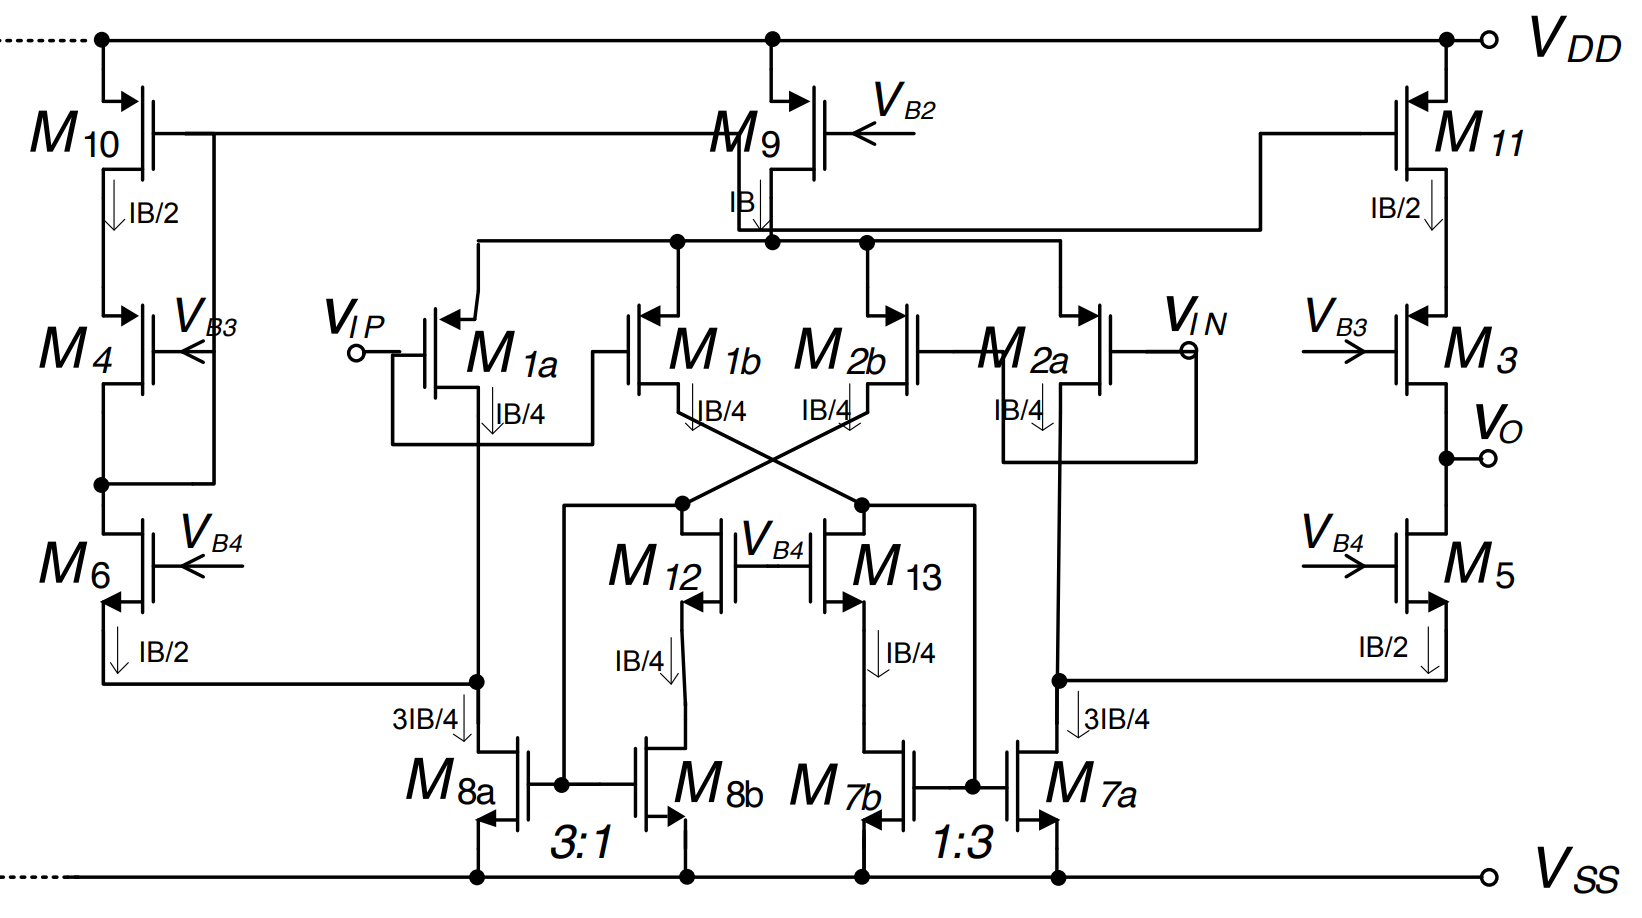
\includegraphics[scale=0.3]{report/Images/RFCA_MAIN.png}
    \caption{Schematic of the Recycling Folded-Cascode Transconductance Amplifier without biasing circuit}
    \label{fig:RFCA_MAIN}
\end{figure}

\textcolor{red}{eventualmente Bonitificar e citar [2]}\\

Based on article [2]:
\begin{itemize}    
    \item M1a, M1b, M2a and M2b are the imput drivers that conduct fixed and equal currents $\frac{I_B}{4}$, corresponding to Vip and Vin respectively. 
    \item M8a, M8b, M7a and M7b are \textit{driver transistors} their role is to provide a folding node for the small signal current generated by the input.
    The current ratio for these current mirrors is 3 so (8a and 7a) transistors have a current of $\frac{3.I_B}{4}$ and (8b and 7b) transistors have a current of $\frac{I_B}{4}$. The cross-over connections of these current mirrors ensure the small signal currents added at the sources of M5 and M6 are in phase
    \item   M12 and M13 are sized similar to M5 and M6, and their addition helps maintain the drain potentials
    of M8a, M8b, M7a and M7b equal for improved matching.
\end{itemize}

\textcolor{red}{Aqui vi no Gepeto pq não diz nada no artigo}
\begin{itemize}    
    \item M5 and M6 are common-source amplifying transistors, they are responsible for converting the differential currents from the folded-cascode stage ( M7a, M7b, M8a, M8b, M11 and M12) into voltage at their drains.
    \item M4 and M3 are current mirror transistors, their main role is to replicate the current from M6 and M5 into the output node.
    \item M10 and M11 act as cascodes for M4 and M3 they help isolate the output node from other circuit dynamics, enhancing stability and bandwidth.\\
    
    (Cascoding improves the overall output impedance by reducing the Miller effect, which minimizes the effect of parasitic capacitances and increases gain. \textcolor{red}{CONFIRMAR ISTO})
 
\end{itemize}
\newpage